\documentclass{ceurart}

\usepackage{hyperref}
\usepackage{subcaption}
\usepackage{changepage,titlesec}
\titleformat{\section}[block]{\Large\bfseries}{\thesection.}{1em}{}
\titleformat{\subsection}[block]{\large\bfseries}{\thesubsection}{1em}{}
\titleformat{\subsubsection}[block]{\bfseries}{\thesubsubsection}{1em}{}
\titlespacing*{\subsection} {2em}{3.25ex plus 1ex minus .2ex}{1.5ex plus .2ex}
\titlespacing*{\subsubsection} {3em}{3.25ex plus 1ex minus .2ex}{1.5ex plus .2ex}


%%
%% end of the preamble, start of the body of the document source.
\begin{document}

%%
%% Rights management information.
%% CC-BY is default license.
\copyrightyear{2022}
\copyrightclause{Copyright for this paper by its authors.\\
  Use permitted under Creative Commons License Attribution 4.0
  International (CC BY 4.0).}

%%
%% This command is for the conference information
\conference{CLEF 2022: Conference and Labs of the Evaluation Forum, September 5--8, 2022, Bologna, Italy}

%%
%% The "title" command
\title{Aldo Nadi at Touch{\'e} 2022: Argument Retrieval for Comparative Questions}

\subtitle{Notebook for the Touch{\'e} Lab on Argument Retrieval at CLEF 2022}

%%
%% The "author" command and its associated commands are used to define
%% the authors and their affiliations.
\author[1]{Maria Aba}[%
email=maria.aba@studenti.unipd.it
]

\author[1]{Munzer Azra}[%
email=munzer.azra@studenti.unipd.it
]

\author[1]{Marco Gallo}[%
email=marco.gallo.9@studenti.unipd.it
]

\author[1]{Odai Mohammad}[%
email=odai.mohammad@studenti.unipd.it
]

\author[1]{Ivan Piacere}[%
email=ivan.piacere@studenti.unipd.it
]

\author[1]{Giacomo Virginio}[%
email=giacomo.virginio@studenti.unipd.it
]

\author[1]{Nicola Ferro}[%
orcid=0000-0001-9219-6239,
email=ferro@dei.unipd.it,
url=http://www.dei.unipd.it/~ferro/,
]

\address[1]{University of Padua, Italy}


%%
%% The abstract is a short summary of the work to be presented in the
%% article.
\begin{abstract}
	In this paper we present the information retrieval system we developed for the 2022 Touché @ CLEF Task~2 evaluation campaign. The participation in the task is performed as a student group project conducted in the Search Engines course a.y. 2021/2022 at the Computer Engineering and Data Science master degrees at University of Padua.\\
	This tasks' aim is to create systems that are able to retrieve documents that compare two options, e.g. which is the best pet between a dog and a cat.\\
	Here we describe the architecture of our system, we list the software and hardware resources we made use of, we discuss the results obtained using different configurations and finally we present improvements which could be applied to our system to enhance its performance.
\end{abstract}

%%
%% Keywords. The author(s) should pick words that accurately describe
%% the work being presented. Separate the keywords with commas.
\begin{keywords}
  Information retrieval \sep
  Comparative questions \sep
  Lucene
\end{keywords}

%%
%% This command processes the author and affiliation and title
%% information and builds the first part of the formatted document.
\maketitle


\section{Introduction}
\label{sec:introduction}

Before the era of the internet, information storage and retrieval systems were mostly
used by professionals for medical research, in libraries, by governmental
organizations, and archives. Therefore, access to such information was a hard process especially
for non-search experts. Recently, with the fast increase in the number of data and information
available online, the importance of search engines grew rapidly. Nowadays, people use
search engines to locate and buy goods, choose a vacation destination, select
a medical treatment, etc. Search engines
transitioned from being searchers' tools for information to tools for building opinions and making
major decisions. All of these aspects, when considered together, make retrieval systems a need for impacting
the industry and improving the field of information retrieval.


This paper is structured as follows: Section~\ref{sec:methodology} describes our
approach; Section~\ref{sec:setup} explains our experimental setup; Section~\ref{sec:results}
discusses our main findings; finally, Section~\ref{sec:conclusion} draws some conclusions and
outlooks for future work.

\vspace{2em}
\section{Related Work}
\label{sec:related work}

The packages mentioned in \ref{subsec:parse, analyze, index} and \ref{subsec:search} are obtained expanding from a baseline built on the TIPSTER collection, during lessons of the "Search Engines" course, University of Padua.\\ Information about the course are available online:
\footnote{\url{https://en.didattica.unipd.it/off/2021/LM/IN/IN2547/004PD/INQ0091599/N0}}

\vspace{2em}
\section{Methodology}
\label{sec:methodology}

The developed Java system is divided into the following packages, each package representing a stage:


\subsection{Parse}
  
  This package is divided into two packages: 
\subsubsection{Document}
        
            The aim of this package of the project is to facilitate the parsing of the document corpus provided by CLEF for the Touchè Task 2 so that they can be used together with Lucene. The corpus for Task 2 is a collection of about 0.9 million text passages contained in a single JSON file passages.json. The file contains several documents organized as nodes of a JSON tree and each node contains 3 different fields. Namely id, contents, and chatNoirUrl. In this project only the id and the contents data of the document are retrieved from the JSON node and used in the implementation. The chatNoirUrl is not taken into account since we found it to not be relevant for the task. Furthermore, CLEF also provided a version of the corpus with text passages expanded with queries generated using DocT5Query. We found this expanded version valuable and added support for parsing it in our implementation. The DocT5Query queries are contained within the 'contents' key of each document. The parsing is implemented in the following classes:
            \begin{enumerate}
                \item 
                    DocumentParser.java: Similar to HelloTiptster’s, the class creates a     document parser that takes a reader object to be used as input, it overrides the hasNext() and next() methods, and performs the actual parsing.
                \item 
                    Parser.java: This is a customized class that specializes the HelloTipster parser used on the TIPSTER corpus by our teacher. It extends the aforementioned DocumentParser class and takes the reader object as input. The hasNext() method has been implemented and it is where the actual parsing takes place and it extracts the three already mentioned fields.
                \item
                    ParsedDocument.java: Represents the actual document to be indexed by Lucene. It defines the id, contents, and docT5Query of the JSON documents. The class defines proper getter and setter methods for the various fields to be easily retrieved and set, and it overrides utility methods like toString(), equals(), and hashCode().
            \end{enumerate}
\subsubsection{Topic}
        
            The aim of this package of the project is to facilitate the parsing of the topics provided by CLEF for the Touchè Task 2 so that they can be used together with Lucene. The topics of Task 2 is a collection of 50 topics contained in a single XML file topics-task2.xml. The file contains the topics each having 5 different attributes. Namely number, title, objects, description, and narrative. In this project, even though all the attributes of a topic are parsed, Only the number, objects, and title are used for search. The narrative and description attributes are used for manual relevance. The parsing is implemented in the following classes:
            \begin{enumerate}
                \item 
                    TopicParser.java: Similar to DocumentParser.java, the class creates a     topic parser that takes a reader object to be used as input, it overrides the hasNext() and next() methods, and performs the actual parsing.
                \item 
                    XMLTopicParser.java: This is a customized class that  extends the aforementioned TopicParser class and takes the reader object as input. The hasNext() method has been implemented and it is where the actual parsing takes place and it extracts the already mentioned fields.
                \item
                    ParsedTopic.java: Represents the actual topic to be used in the searcher with Lucene. It defines all the attributes of a topic. The class also defines proper getter and setter methods for the various fields to be easily retrieved and set, and it overrides utility methods like toString(), equals(), and hashCode().
            \end{enumerate}
\subsection{Analyze}
  
    We have built three analyzers, to process the documents, perform tokenization and use different combination of filters.
\subsubsection{AnalyzerUtil.java}
            
            This is a helper class auxiliary class containing utility methods for loading stop lists in the resource folder. These stop lists were obtained from well-known standard lists based off high frequency words. Some of them are: Atire, Indri, Smart, Terrier, Zettair, Glasgow, Snowball, Okapi, and Lucene. 
\subsubsection{BaselineAnalyzer.java}
            
            This is a java class for tokenization which starts with a StandardTokenizer ad reducing every word to lower case using a LowerCaseFilter and then we have used the StopFilter to remove frequent words in the collection that do not bring useful information. 
\subsubsection{MainAnalyzer.java}
            
            Contains various filters from AnalyzerUtil as well as EnglishPossessiveFilter and MultipleCharsFilter. It also adds synonyms dictionary to perform a query expansion based on Wordnet.
\subsection{Index}
  
     This package contains the 3 classes responsible for the index creation, they are as follows: 
     
\subsubsection{BodyField.java}
    
        Represents the body of a specific document it has two different constructors, one accept a Reader and the other accept a String value. The only field is BODY\_TYPE  which is tokenized and not stored, keeping only document ids and term frequencies in order to minimize the space occupation. 
\subsubsection{DirectoryIndexer.java}
    
        It's used for indexing the whole directory tree, it takes as parameter the Analyzer to be used, the Similarity, the size in megabytes of the buffer for indexing documents, the directory where to store the index, the directory from which documents have to be read, the extension of the files to be indexed, the charset used for encoding documents, the total number of documents expected to be indexed and the class of the DocumentParser to be used. The constructor take these handles several exception that may rise and take care of the index writer configuration. For testing purposes we added a main method which create a new DirectoryIndexer using custom parameters and than run the method index which do the actual indexing of the documents and skip every file which doesn't have the correct extension, important to note the fact that we added a new custom parameter DocT5QueryField. 
\subsubsection{DocT5QueryField.java}
    
        It manages the new tokenized and not stored field for the document, differently from the body field this class has only one constructor which accepts Strings.
\subsection{Search}
  
  The search package contains just the Searcher class. This class is responsible for:
    \begin{enumerate}
    	\item Retrieving and preparing the topics for the search.
    	
    	The topics are retrieved directly from the topics file and parsed using the XMLTopicParser class.
    	Then an Analyzer is defined to tokenize and filter the tokens before the search.
    	\item Defining how to use topics in the search.
    	
    	We decided to use just the topics titles in the search by similarity, but we used the topic objects (the items which the user wants to compare) as a filter: we selected among the search results just those that presented both the terms.
    	Moreover we made it possible to assign weights to the different fields of the documents among which to search, or to select just one of the two fields.
    	\item Defining which type of comparison to perform between topics and documents.
    	
    	The searcher class accepts as a parameter a similarity function to compare the two.
    	\item Writing the results on a file
    \end{enumerate}

    We experimented with different configurations. We especially tried changing:
    \begin{itemize}
    	\item Similarity functions
    	\item Whether we applied filtering or not to the search results
    	\item Analyzer, in particular the stoplist it uses
    \end{itemize}
\subsection{RF}
  
      This package contains a single class, also called RF.
        
        RF.java is a customized class with the goal of performing a search using relevance feedback to perform query expansion.
        
        RF functions in a similar way to the Searcher class, with the exception of building the query used in the searching using the tokens present in relevant documents, instead of using the terms in title field of the topics file.
        
        The class collect all docID and relevance of relevant documents in the \textit{qrels} file.
        
        The tokens and their frequency in the relevant documents are retrieved by searching the document by docID and iterating through its termvector.
        
        The tokens used in the search are boosted by their frequency in the document multiplied by the square of the relevance score.
        
        Relevance Feedback is standardly based on the Rocchio Algorithm.
        The formula for the Rocchio Algorithm is:
        $$
        \overrightarrow{Q_{m}}=
        \left(a\cdot\overrightarrow{Q_{O}}\right)+
        \left(b\cdot\frac{1}{|D_{r}|}\cdot\sum_{\overrightarrow{D_{j}}\in D_{r}}\overrightarrow{D_{j}}\right)-
        \left(c\cdot\frac{1}{|D_{nr}|}\cdot\sum_{\overrightarrow{D_{k}}\in D_{nr}}\overrightarrow{D_{k}}\right)
        $$
        where $\overrightarrow{Q_{m}}$ is the modified query vector, $\overrightarrow{Q_{O}}$ is the original query vector, $\overrightarrow{D_{i}}$ is the document vector for the $i^{th}$ document, $D_{r}$ is the set of relevant documents, $D_{nr}$ is the set of non-relevant documents and $a$, $b$ and $c$ are weight parameters.
        
        In our case the parameters used are 0, 1, 0.
        Rocchio algorithm is written for binary relevance, our version of RF is customized to take into account the different relevance scores used in this test collections (0 to 3).
        
        The results of the search are then outputted as a standard run file.
        
\subsection{RRF}
  
      This package contains a single class, also called RRF.
        
        RRF.java is a customized class with the goal of performing using Reciprocal Ranking Fusion to fuse the results of different runs in a single one.
        
        RRF takes in imput a directory path and performs RRF using all the runs in .txt documents inside that directory.
        
        For each documents and for each topic the documents and their respective ranking are collected.
        
        Then document receive a new scoring using the RRF formula.
        
        Given a set of documents \textit{D} and a set of rankings \textit{R} for the documents, the formula for RRF is:
        $$RRFscore(d \in D)=\sum_{r \in R}^{}\frac{1}{k+r(d)}$$
        where k is a fixed number, in this case k is set to 30.
        
        Then, for each topic, documents are ranked (and ordered) based on their RRF score.
        
        The results of the search are then outputted as a standard run file.
\subsection{Filter}
 
    The main filter class contains two methods responsible for adding the term to the search object. The main method is filterAnd it takes two parameters as input: a query parser object to convert the string into meaning full term for the search method. And a String s represents the term that needed to add to the query parser It will return an object of BooleanQuery.Builder which can be consumed later by the search method. The second method is just a helper method to extract the string object from the "objects field", tokenized the sentences, and remove any unwanted characters.

\subsection{Argument quality}
  
  We decided to make use of IBM Project Debater API.
  
      Project Debater is an AI system used to perform various tasks about debating at a human level. IBM makes freely available, for research purposes, some services bases on this system through an API. \citep{ProjectDebaterAPI}
      
      We were interested in the argument quality service of the API. It accepts a couple of strings labeled as Sentence and Topic, and it returns a float score in the range 0-1 based on the relevance of the sentence for the topic and on the quality of the sentence as a text, which means how good it is written. We were not interested in the first part of the evaluation because the rest of our system was designed to do that, so it would be redundant. We just wanted to evaluate the text quality. So we decided to send Sentence-Topic pairs in which the Topic part was an empty string.
      
      We coded the ArgumentQualityVerifier class which evaluates the written quality of each document by using the API and then saves the scores to a file.
      
      Then we had to use the obtained scores to rerank the results of the search saved in a run file. So we defined the ArgumentQualityReranker class which:
      
       \begin{enumerate} 
           \item loads the quality scores of all the documents from the file into a Map object \item iterates over the lines of the old run file, multiplies the old score by the one assigned by Project Debater API and saves the object representing the new line to a list \item sorts the list of new lines by topic number and score and writes them on a new run file 
       \end{enumerate}

\subsection{Run.java}

The developed Java system also contains the class Run.java. This is the main class used for running the entire system. It accepts the following parameters: 

    \begin{enumerate}
        \item Task
            
            Specifies which stage to be run.
            
            Possible values: 'parse', 'index', or 'search'.
    
            Default value = 'index'
        \item indexDirectoryPath
            
            Specifies the location of index files.
            
            Possible values: the path to the index.
            
            Default value = 'experiment/index'
        \item stopListFilePath
            
            Specifies the location of the stop list file to use.
        
            Possible values: the path to the stop list file to be used.
            
            Default value = 'lucene.txt'
        \item filter
            
            Specifies whether or not to filter by topic objects during search
            
            Possible values: 'true', 'false'.
            
            Default value = 'false'
        \item matching
            
            Specifies the type of similarity to use.
            
            Possible values: 'bm25', 'tfidf', 'lmd'.
            
            Default value = 'bm25'
        \item runId
            
            Specifies the ID of the run.
            
            Possible values: any string.
            
            Default value = 'seupd2122-kueri'
        \item runDirectoryPath
            
            Specifies the directory  to which to write runs.
            
            Possible values: any valid directory path.
            
            Default value = 'runs'
        \item qrelFilePath
            
            Specifies the directory to which to write qrels of RF search.
            
            Possible values: any valid directory path.
            
            Default value = 'code/src/main/resource/qrels/example.txt'

\end{enumerate}

Following is the class diagram for our implementation

\begin{figure}[h]
\centering
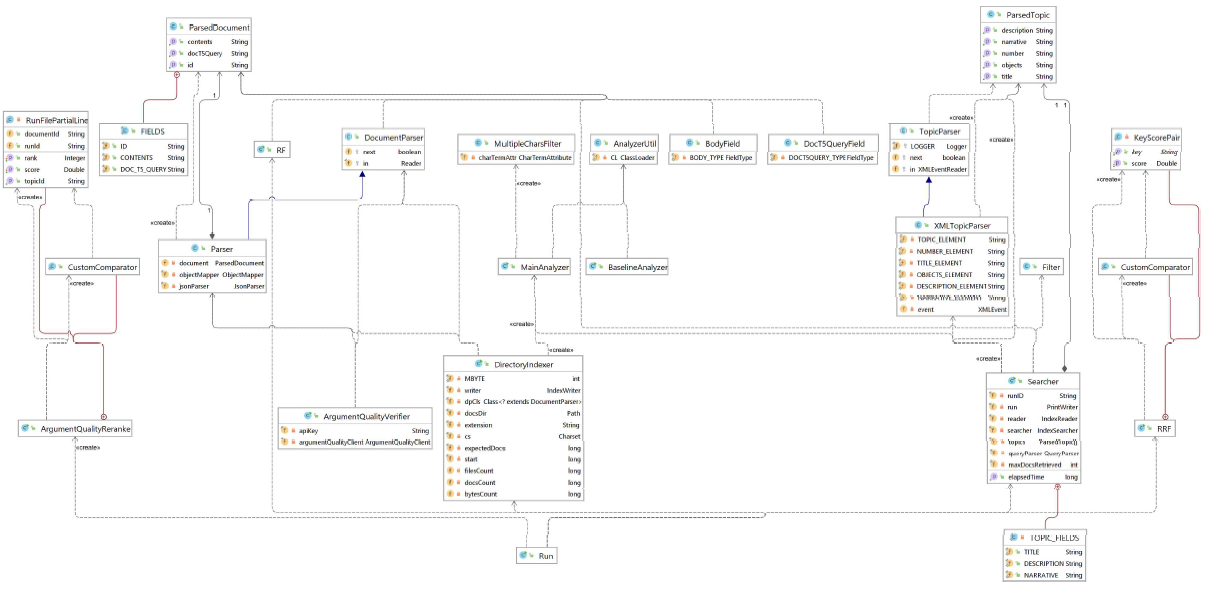
\includegraphics[width=\textwidth]{figure/class-diagram.PNG}
\caption{Class diagram of the project}
\end{figure}

\vspace{2em}
\section{Experimental Setup}
\label{sec:setup}

\subsection{Collections}

	Some of the collections used throughout the process of system development were the ones provided by CLEF for the Touché 2022 edition, accessible from Task~2's site. Those include:

	\begin{itemize}
		\item topics-task2.xml which contains the topics.
		\item The original version of passages.jsonl which contains the documents.
		\item DocT5Query expanded version of passages.jsonl\footnote{This collection was provided by Team Princess Knight that parteciped in Touche, the corpus can be found at: \url{https://www.tira.io/t/expanded-passages-for-the-touche-22-task-2-argument-retrieval-for-comparative-questions/578}} which contains the documents expanded with queries generated using DocT5Query. \citep{nogueira:2019}
	\end{itemize}

	Other collections are:
	\begin{itemize}
		\item Historical stoplists: lucene, smart and terrier;
		\item Custom stoplists:
			\begin{itemize}
				\item Kueristop - Stoplist formed by the 400 most concurrent term in the Contents field of the document collection;
				\item Kueristopv2 - Subset of kueristop, obtained by removing from it terms appearing in the Objects field of the topics, except for the very general terms also appearing in lucene stoplist ("in" and "the").
			\end{itemize}
		\item Sentence quality - file containing, for each document in the document Collection, the pairs of docIds and the score obtained by that document as explained in \ref{subsec:Argument quality}.
	\end{itemize}
	

\subsection{Evaluation measures}

	The evaluation measure used is Normalized Discounted Cumulative Gain at depth 5, NDCG@5 in short. \citep{jarvelin:2002}

	It is the evaluation measure used by Touché to officially evaluate runs.

	NDCG@k is calculated as follows:

	$$
	NDCG@k = \frac{DCG@k}{iDCG@k}
	$$
	where
	$$
	DCG@k = \sum_{i=1}^{k}\frac{relevance_i}{log_2(i+1)}
	$$
	and iDCG@k is the ideal DCG@k, meaning the DCG@k for documents ordered by relevance, highest to lowest.


\subsection{Git repository}

	The project’s development can be found in the following link to its Git repository  \footnote{\url{https://bitbucket.org/upd-dei-stud-prj/seupd2122-kueri/src/master/}}
	

\subsection{Hardware}

	The specifications of the computer used to perform the runs are the following:
	\begin{description}
		\item[OS] Windows 10 Home 21H2 x64
		\item[CPU] AMD Ryzen 5 1600 @ 3.9GHz
		\item[RAM] 16GB 3000mhz cl16
		\item[GPU] Nvidia GTX 1060 6GB
		\item[HDD] 2TB 7200RPM
	\end{description}

\vspace{2em}
\section{Results and Discussion}
\label{sec:results}

The conventional and ideal approach when evaluating the performance of the runs would have been to use last year's test collection. However, since we did not have access to last year's corpus we have decided to use this year's test collection to evaluate our systems, using a \textit{qrels} file containing relevance feedback manually performed by us.

The \textit{qrels} file has been built by gathering, for each of the runs performed, the top 5 ranked documents for each topic.

The runs' performance has been evaluated using \textit{trec\_eval}, the key measures considered are \textit{NDCG@5}, the official measure used by CLEF to rank runs, and \textit{num\_q}, the number of topics retrieved (since some runs retrieved no documents for some of the topics).

All the runs, their characteristics and key measures are reported in Table \ref{tab:results-table} and \ref{tab:results-rrf-table}. The five runs with their number in bold are the five submitted runs.

All the runs are performed on indexes obtained using Standard tokenizer and Lowercase filter, except for indexes used in runs obtained using Relevance Feedback, which use Letter tokenizer instead; this is because some of the tokens obtained using standard tokenizer were written in a format that caused errors when used as query (e.g. "text:text:text" would be a token that caused errors).

\begin{table}[t]
	\caption{NDCG@5 and setup for single runs}
	\label{tab:results-table}
	\centering
	\begin{tabular}{|c||c|c||c|c|c|c|c|c|c|}
		\toprule
		\# & NDCG@5 & num\_q  & RF & Stoplist & Filter & Stemmer & Similarity & Weights & Reranking \\
		\midrule
		1 & 0.3830 & 50 & False & lucene & False & None & BM25 & [1,1] & False \\
		2 & 0.3756 & 50 & False & lucene & False & None & LMD & [1,1] & False \\
		3 & 0.3313 & 50 & False & lucene & False & None & TFIDF & [1,1] & False \\
		\hline
		4 & 0.4140 & 50 & False & smart & False & None & BM25 & [1,1] & False \\
		5 & 0.4258 & 50 & False & terrier & False & None & BM25 & [1,1] & False \\
		6 & 0.4366 & 50 & False & kueristop & False & None & BM25 & [1,1] & False \\
		7 & 0.4548 & 50 & False & kueristopv2 & False & None & BM25 & [1,1] & False \\
		\hline
		8 & 0.4015 & 48 & False & lucene & True & None & BM25 & [1,1] & False \\
		9 & 0.4759 & 41 & False & kueristop & True & None & BM25 & [1,1] & False \\
		10 & 0.4823 & 48 & False & kueristopv2 & True & None & BM25 & [1,1] & False \\
		\hline
		11 & 0.2634 & 50 & False & kueristopv2 & False & None & BM25 & [0,1] & False \\
		12 & 0.3654 & 50 & False & kueristopv2 & False & None & BM25 & [1,0] & False \\
		13 & 0.4525 & 50 & False & kueristopv2 & False & None & BM25 & [1,2] & False \\
		14 & 0.4674 & 50 & False & kueristopv2 & False & None & BM25 & [2,1] & False \\
		\hline
		\textit{\textbf{15}} & 0.4873 & 50 & False & kueristopv2 & False & Porter & BM25 & [1,1] & False \\
		\hline
		16 & 0.8549 & 50 & True & kueristopv2 & False & False & BM25 & [1,1] & False \\
		17 & 0.8552 & 50 & True & kueristopv2 & False & Porter & BM25 & [1,1] & False \\
		\hline
		18 & 0.5867 & 48 & False & kueristopv2 & True & None & BM25 & [1,1] & True \\
		19 & 0.5392 & 50 & False & kueristopv2 & False & None & BM25 & [2,1] & True \\
		\textit{\textbf{20}} & 0.5714 & 50 & False & kueristopv2 & False & Porter & BM25 & [1,1] & True \\
		\textbf{21} & 0.8606 & 50 & True & kueristopv2 & False & False & BM25 & [1,1] & True \\
		22 & 0.8323 & 50 & True & kueristopv2 & False & Porter & BM25 & [1,1] & True \\
		\bottomrule
	\end{tabular}
\end{table}

\begin{table}[t]
	\caption{NDCG@5 and setup for rrf runs}
	\label{tab:results-rrf-table}
	\centering
	\begin{tabular}{|c|c|c|}
		\toprule
		\# fused & NDCG@5 & Reranking \\
		\midrule
		\textit{\textbf{10,14,15,16,17}} & 0.7521 & False \\
		\textit{\textbf{10,14,15,16,17}} & 0.7450 & True \\
		\bottomrule
	\end{tabular}
\end{table}

\begin{itemize}
\item The runs 1 to 3 compare BM25, Dirichlet and TFIDF Similarity as scoring functions, using lucene stoplist.
The run using BM25 was the best performer, so we decided to use this Similarity for all the other experiments.

\item Runs 1 and 4 to 7 compare different stoplists, in particular we compared lucene, smart and terrier stoplists and our own custom stoplists kueristop and kueristopv2; the results show that among the "generic" stoplists the larger ones have a bigger impact, but custom stoplists bring to even better improvements, with kueristopv2 being the best.

\item We then wanted to assess the impact of filtering the runs by all the terms in the object field.
Runs 8, 9 and 10 are performed adding the filter to the setup of runs 1, 6 and 7.
Run 9 only retrieved documents for 41 topics, as 9 topics contain, in the ojects field, terms that are in the stoplist (and therefore are in the index); runs 8 and 10 retrieve documents for 48 queries, because lucene and kueristopv2 contain the terms "the" and "in", which again are in the objects field for two queries.
The runs with filtering have a better \textit{NDCG@5} score compared to runs without, however they retrieve less topics. Retrieving no documents for some topics make us assess these runs as worse performing compared to the ones without filtering. Moreover the improvement in \textit{NDCG@5} score could be caused in part by the lack of these topics, as the system could have worse performance for these topics compared to the others.
Despite having worse results when taken singularly, runs using filtering can be used to improve other runs by using \textit{RRF}.

\item Runs 11 to 14 use the same setup as the current best performing run, 7, changing the weight of Contents and DocT5Query fields respectively.
When searching on a single field (weight 0 on the other field) the score is much worse, increasing the weight of DocT5Query field slightly worsens the score, increasing the weight of Contents field instead improve the score.

\item Run 15 adds to the setup of run 7 a stemmer, specifically Porter stemmer; this addition brings to a good improvement in performance.

\item Runs 16 and 17 instead are performed using Relevance Feedback, respectively without stemmer and with Porter stemmer; These runs have an NDGC@5 score incredibly higher than the previous ones, this however is due to using the same collection, and in particular the same \textit{qrels}, to obtain the RF runs and to score its performance.
To have a more reliable assessment of performance we could have done the search on a index built removing documents present in the qrels file. However, while this would have prevented the overfitting problem, we still couldn't have directly compared results to other runs; in fact, the documents in the \textit{qrels} file, being the top documents retrieved, should be the most relevant, which mean we should have expected worse results by the runs performed when removing the documents from the collection.

\item The first \textit{rrf} run is obtained fusing a mixture of well performing and slightly different runs: 10, 14, 15, 16 and 17. It presents a very good NDCG@5 score, but since it uses \textit{RF} runs the score is not reliable as these runs also may contain overfitting.

\item Runs 18 to 22 and the second \textit{rrf} run are obtained by applying reranking to the runs above (10, 14, 15, 16 and 17 and their fusion).
Comparing to their non-reranked respectives we can see that results on RF and rrf runs are mixed, but again not the most reliable because of previous overfitting; on the other three runs instead reranking offers a really great improvement in performance.

\end{itemize}

\vspace{2em}
\section{Conclusions and Future Work}
\label{sec:conclusion}

Provide a summary of what are the main achievements and findings. 

Discuss future work, e.g. what you may try next and/or how your approach could be further developed.

%% Define the bibliography file to be used

\vspace{2em}
\bibliography{bibliography,proceedings,references}


\end{document}
